\section{Depicting non-Euclidean spaces}
One of the main features of the game is the ability to explore non-Euclidean spaces.
To assess our depictions of non-Euclidean spaces, we decided to compare them with the ones from the game \textit{Hyperbolica}\footnote{\url{https://codeparade.itch.io/hyperbolica}} by \textit{CodeParade}.
It should be noted that the approach used in our game, although relatively simple makes it impossible to capture some of the interesting properties of non-Euclidean geometry, like tiling the plane with right-angled regular pentagons in hyperbolic space.

\subsection{Hyperbolic space}
From the visual standpoint, the hyperbolic space can be identified by the fact that the otherwise flat terrain appears "curved downward".
This may create an illusion that the terrain is wrapped around a giant sphere.
However, by exploring the hyperbolic space, we can quickly notice that it is infinite, just like the Euclidean space.
\autoref{fig:hyperbolic-space-games} shows the comparison of the depictions of hyperbolic space between our game and \textit{Hyperbolica}.
\begin{figure*}[h]
    \centering
    \begin{subfigure}[b]{0.475\textwidth}
        \centering
        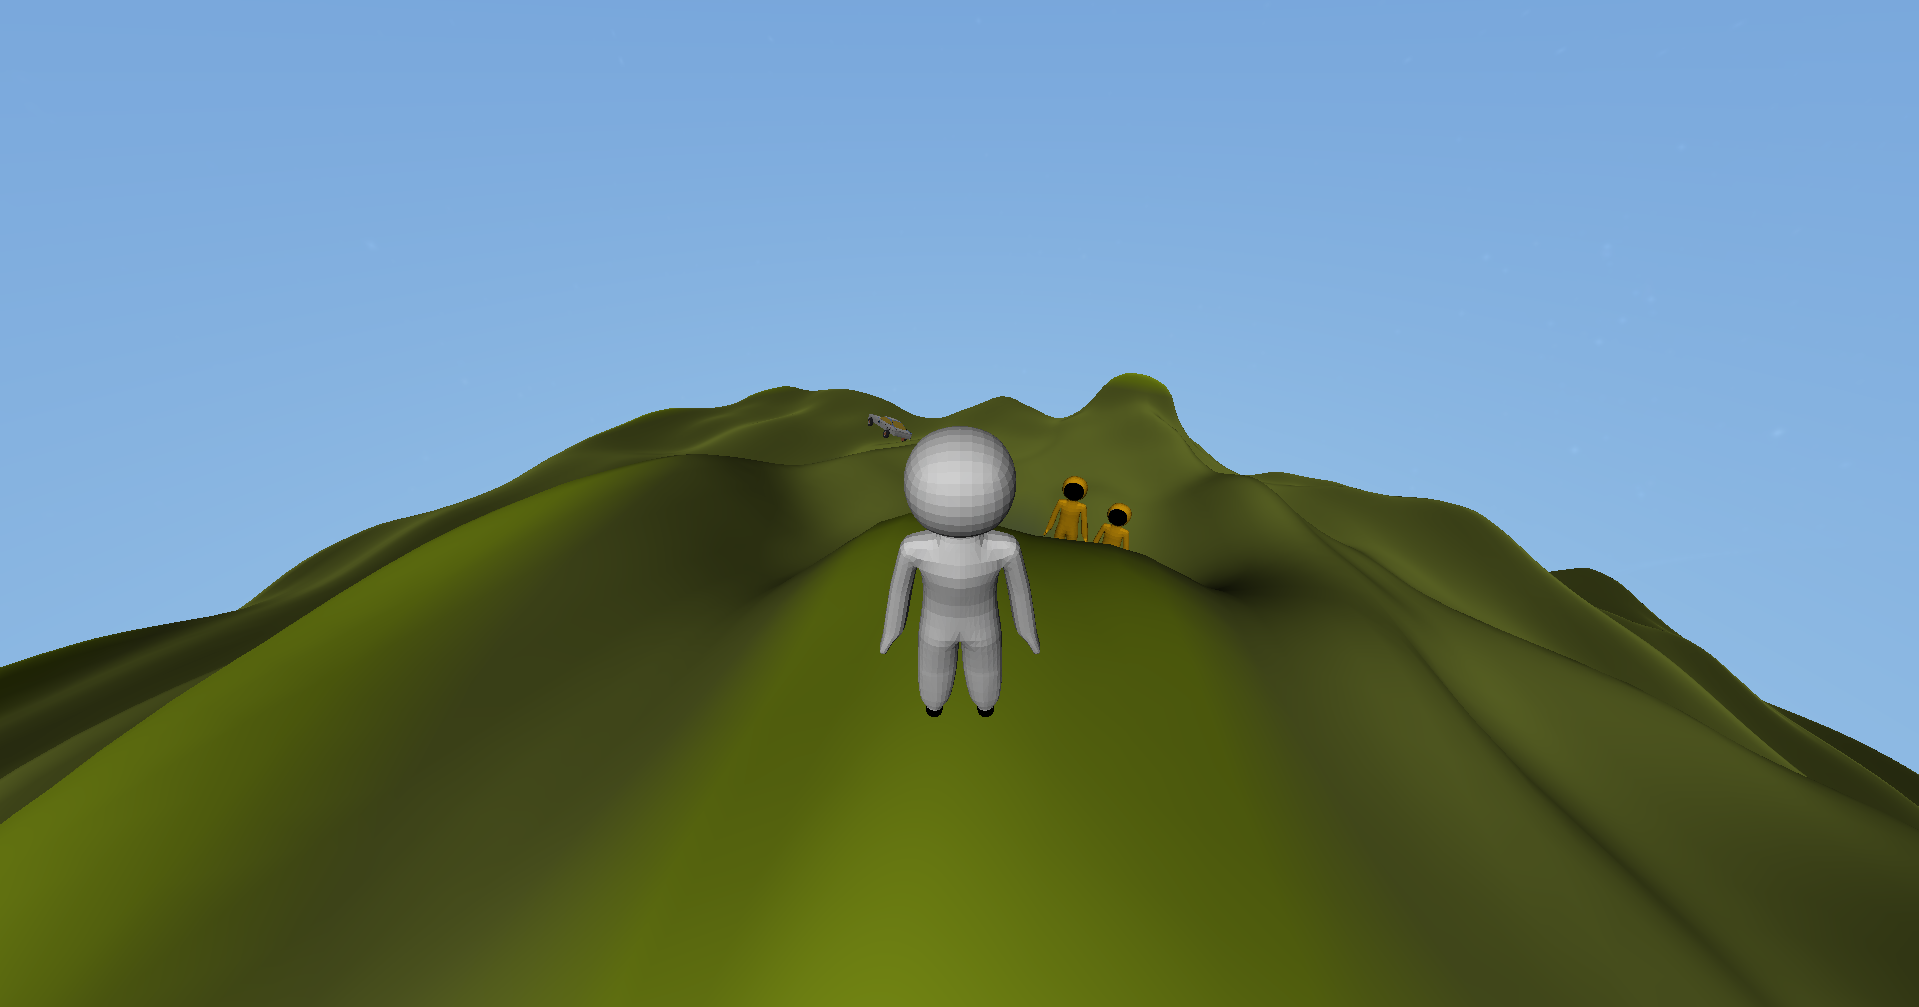
\includegraphics[width=\textwidth]{chapters/results/sections/non_euclidean/resources/hyperbolic-in-hyper.png}
        \caption[]%
        {{\small \textit{Hyper}}}
        \label{fig:hyperbolic-space-games-hyper}
    \end{subfigure}
    \hfill
    \begin{subfigure}[b]{0.475\textwidth}
        \centering
        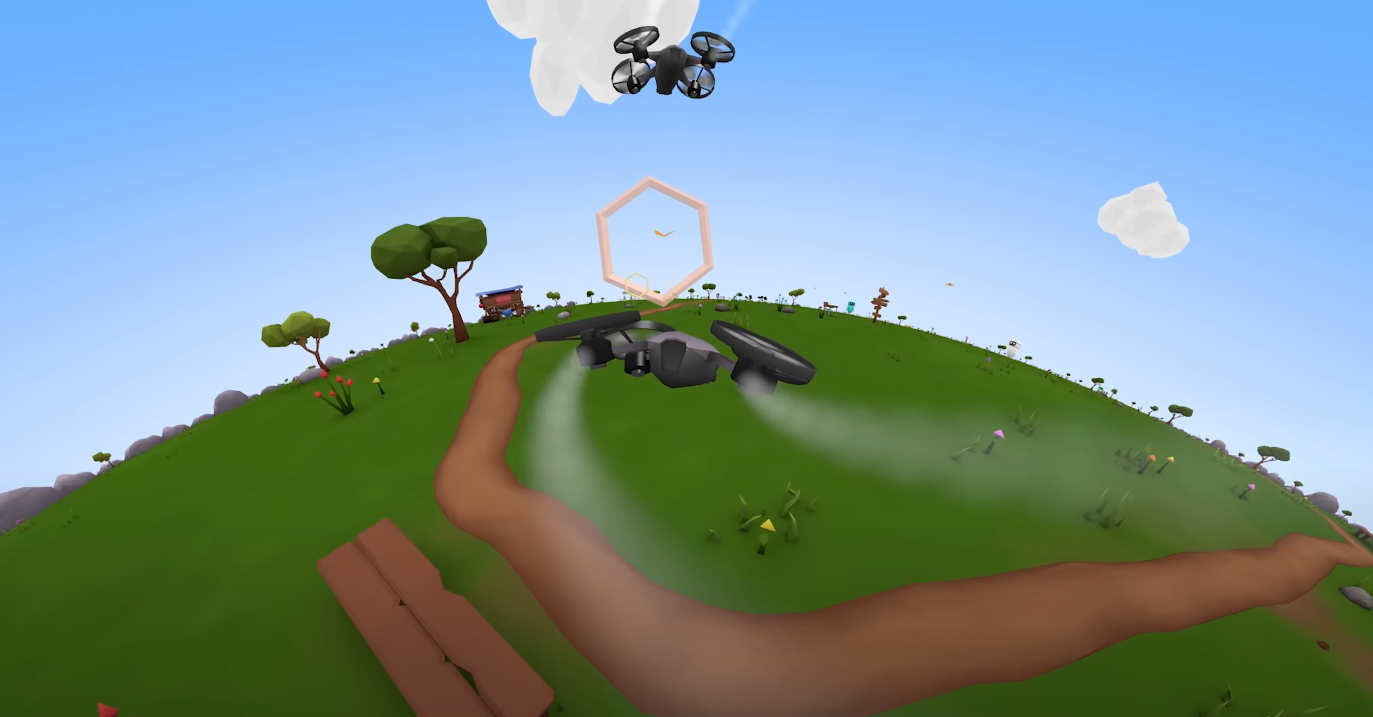
\includegraphics[width=\textwidth]{chapters/results/sections/non_euclidean/resources/hyperbolica-hyperbolic.png}
        \caption[]%
        {{\small \textit{Hyperbolica \cite{Hyperbolica-Hyperbolic}}}}
        \label{fig:hyperbolic-space-games-hyperbolica}
    \end{subfigure}
    \caption[]
    {\small Hyperbolic space}
    \label{fig:hyperbolic-space-games}
\end{figure*}

As mentioned in \autoref{subsubsec:practical-considerations-hyperbolic-space} in our approach the camera's position (as passed to the view matrix) is fixed.
Changing the point where it is located allows us to change the curvature of the terrain.
\autoref{fig:hyperbolic-space-curvatures} shows the scene in hyperbolic space where the camera is positioned close to the origin (cf. \autoref{fig:hyperbolic-space-small-curvature}) resulting in small curvature as compared to the scene when the camera is moved farther from the origin (cf. \autoref{fig:hyperbolic-space-big-curvature}).
\begin{figure*}[h]
    \centering
    \begin{subfigure}[b]{0.475\textwidth}
        \centering
        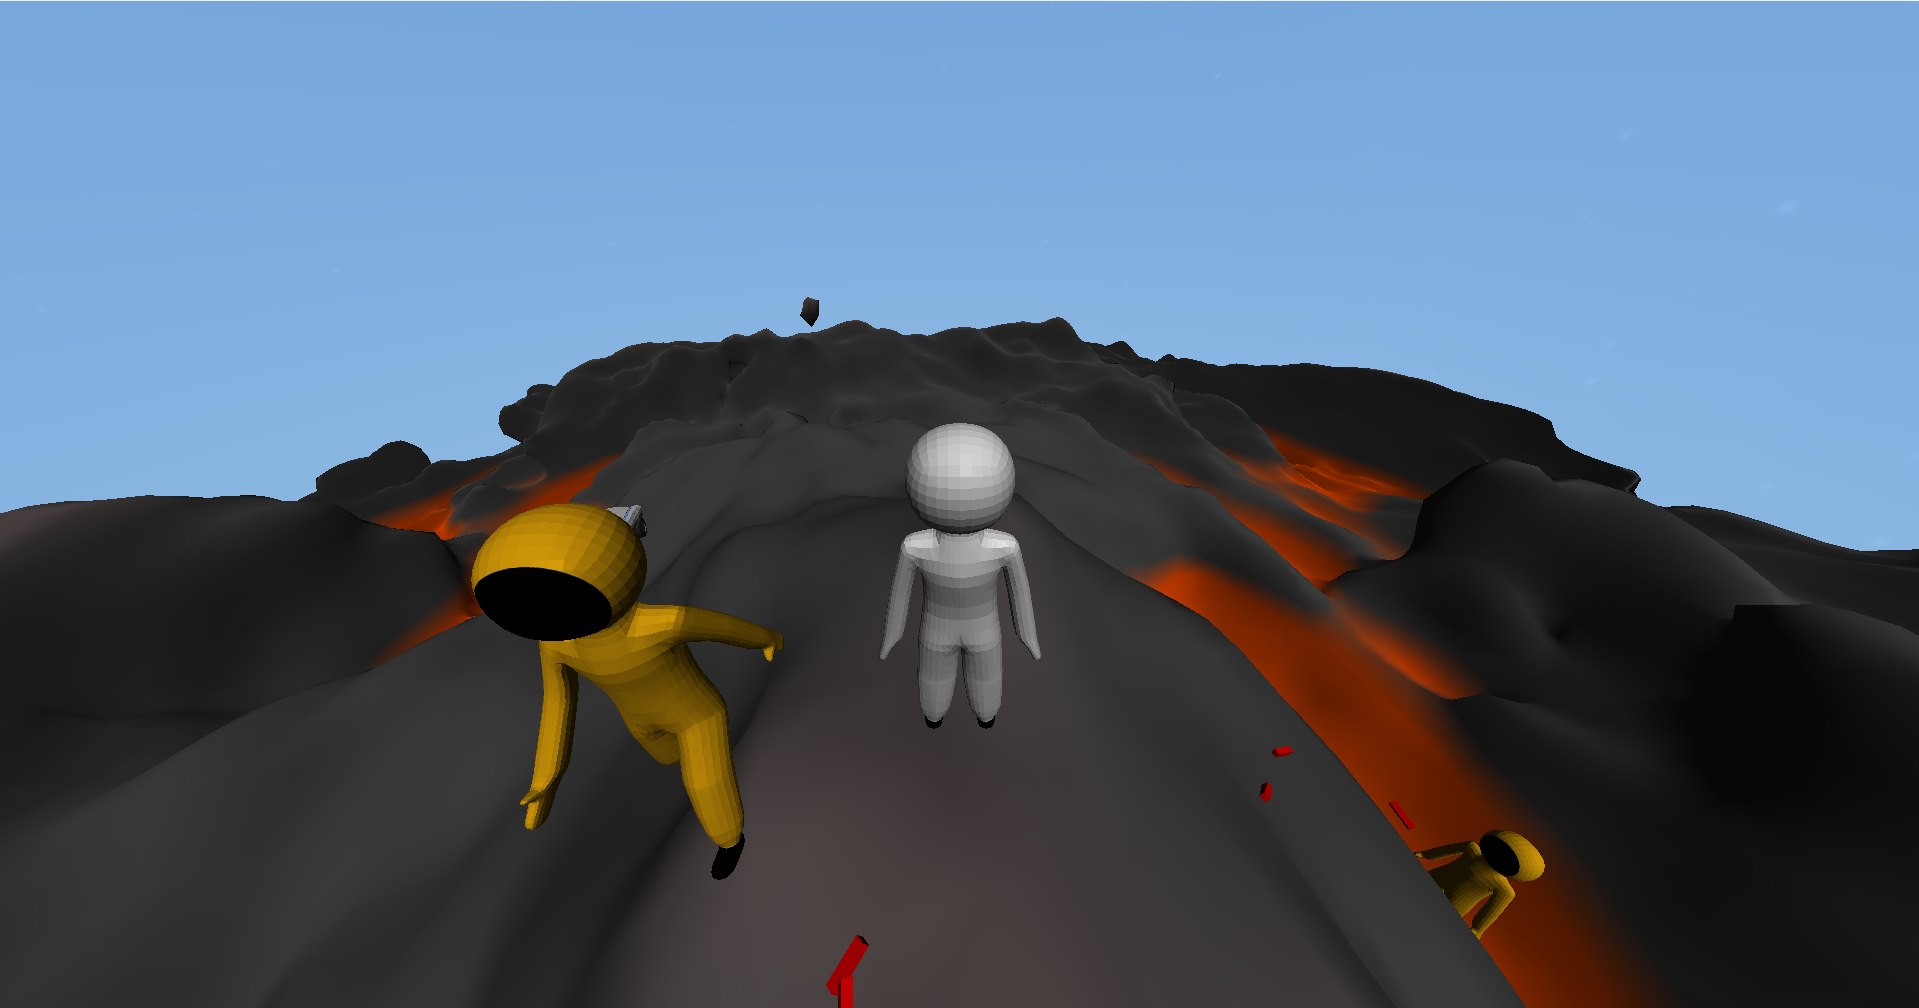
\includegraphics[width=\textwidth]{chapters/results/sections/non_euclidean/resources/hyperbolic-small-curvature.png}
        \caption[]%
        {{\small Camera close to the origin}}
        \label{fig:hyperbolic-space-small-curvature}
    \end{subfigure}
    \hfill
    \begin{subfigure}[b]{0.475\textwidth}
        \centering
        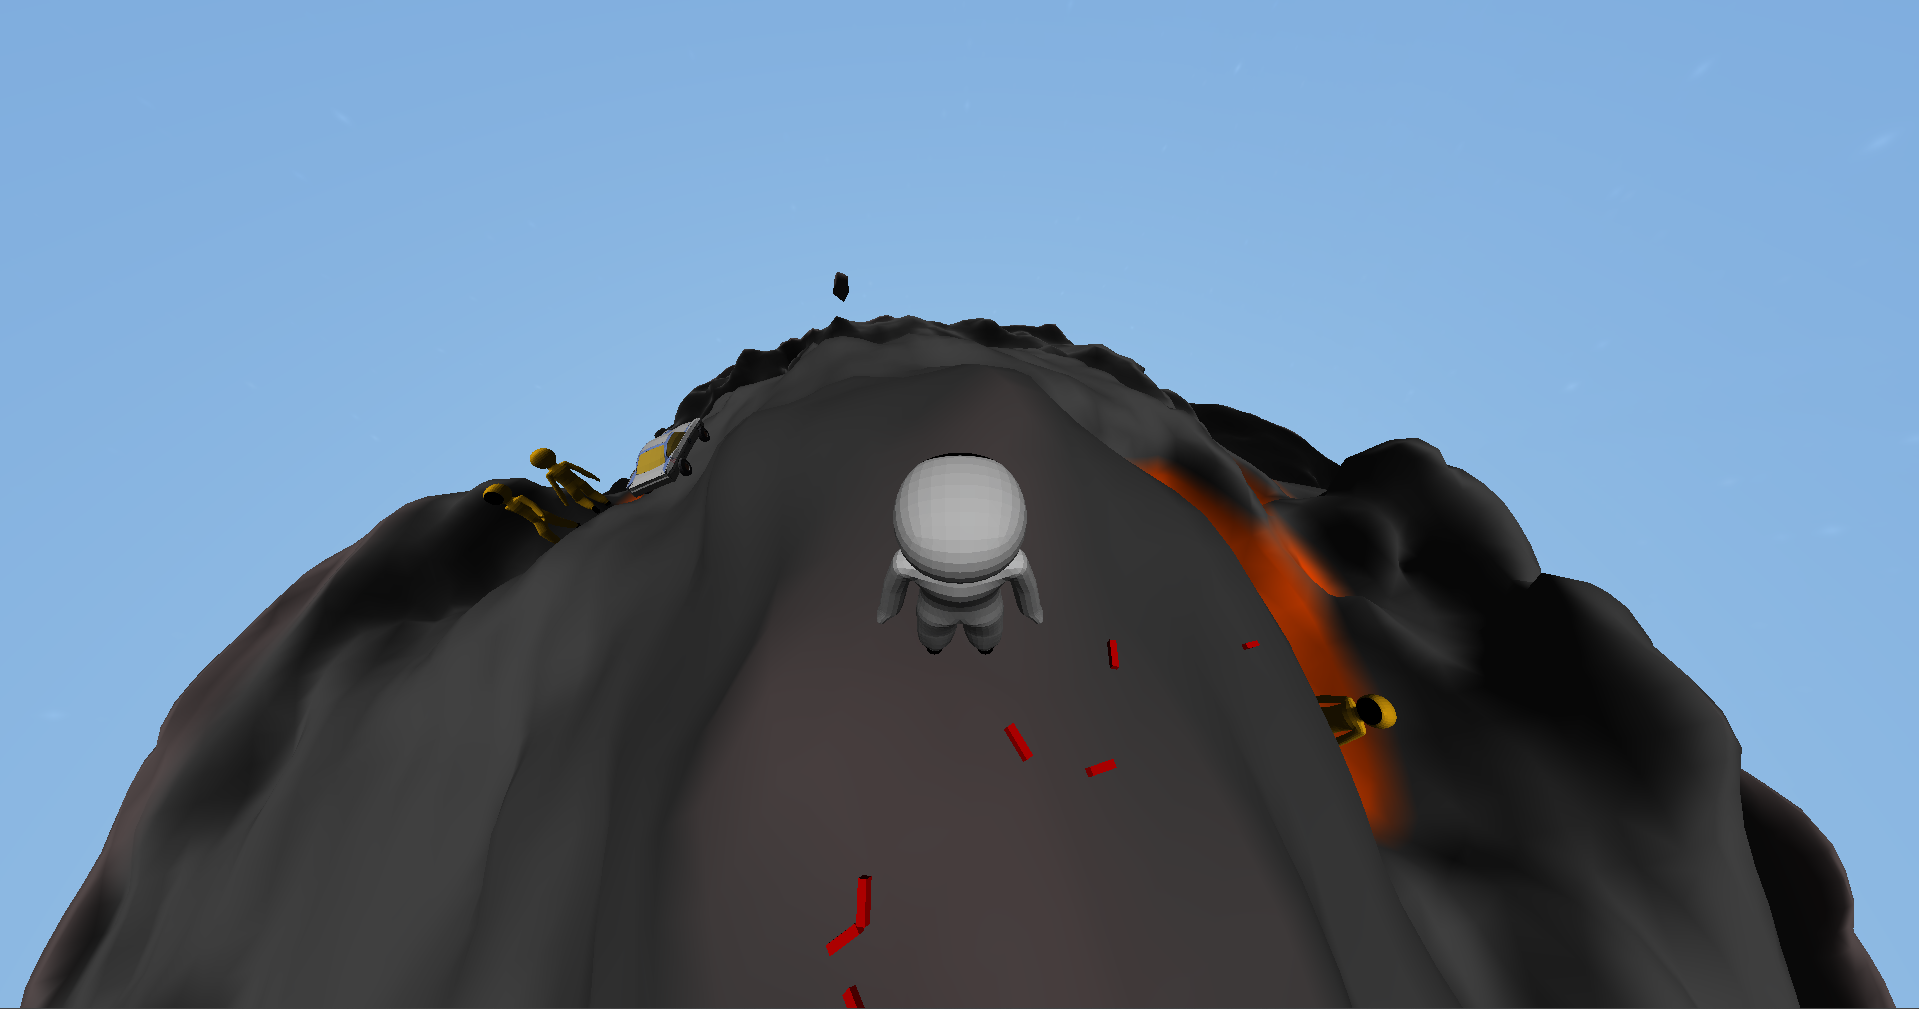
\includegraphics[width=\textwidth]{chapters/results/sections/non_euclidean/resources/hyperbolic-large-curvature.png}
        \caption[]%
        {{\small Camera far from the origin}}
        \label{fig:hyperbolic-space-big-curvature}
    \end{subfigure}
    \caption[]
    {\small Hyperbolic space, different curvatures due to camera's position}
    \label{fig:hyperbolic-space-curvatures}
\end{figure*}

\question{Do we have to mention that our non-Euclidean spaces are "fake" in the sense that you don't have 5-sided right pentagons.}
\subsection{Spherical space}
Playing the video game in spherical space gives the impression that the terrain is wallpapered onto the inside of a giant sphere.
Unlike the hyperbolic space, the spherical space is finite.
Comparison in \autoref{fig:spherical-space-games} shows that our implementation provides visual effects to a certain degree similar to those in \textit{Hyperbolica}.
\begin{figure*}[h]
    \centering
    \begin{subfigure}[b]{0.475\textwidth}
        \centering
        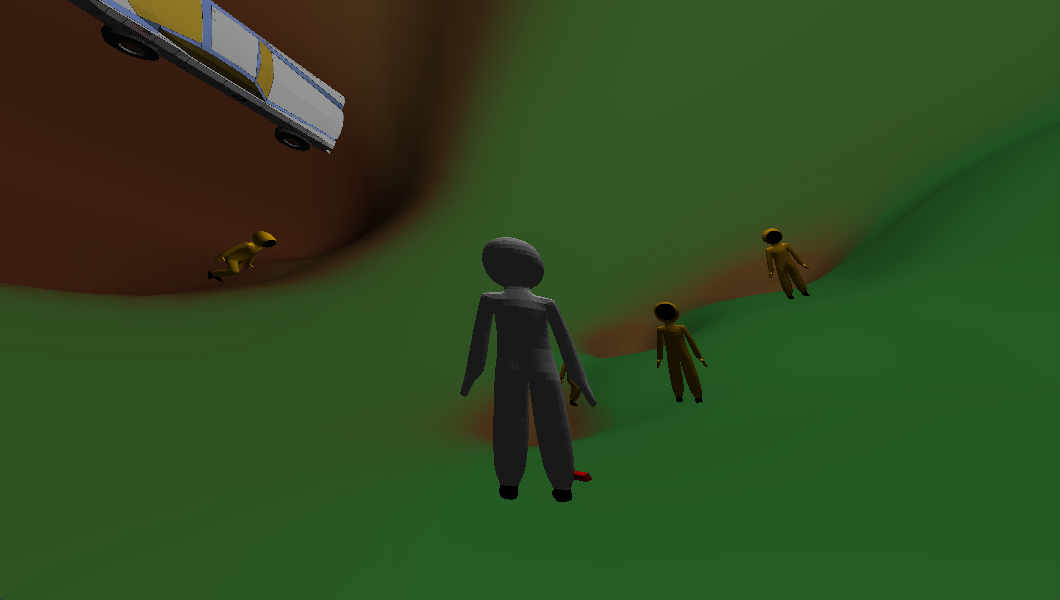
\includegraphics[width=\textwidth]{chapters/results/sections/non_euclidean/resources/spherical-in-hyper.png}
        \caption[]%
        {{\small \textit{Hyper}}}
        \label{fig:spherical-space-games-hyper}
    \end{subfigure}
    \hfill
    \begin{subfigure}[b]{0.5\textwidth}
        \centering
        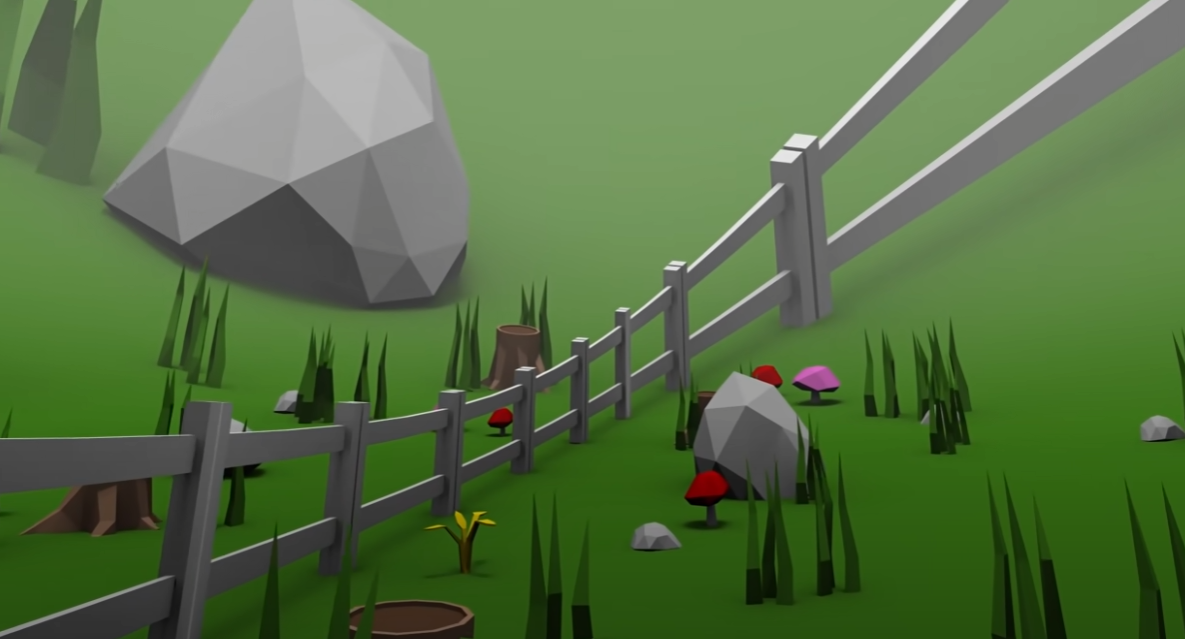
\includegraphics[width=\textwidth]{chapters/results/sections/non_euclidean/resources/hyperbolica-1.png}
        \caption[]%
        {{\small \textit{Hyperbolica \cite{Hyperbolica-Spherical}}}}
        \label{fig:spherical-space-games-hyperbolica}
    \end{subfigure}
    \caption[]
    {\small Spherical space}
    \label{fig:spherical-space-games}
\end{figure*}